\documentclass[a4paper,norsk]{article}
\usepackage[utf8]{inputenc}
\usepackage[T1]{fontenc,url}
\usepackage{babel,textcomp}
\usepackage{graphicx, wrapfig}
\usepackage{graphics}
\usepackage{amsmath}
\usepackage{stackengine}
\usepackage{listings}
\usepackage{amsfonts}
\urlstyle {sf}
\title {A little bit about Random Forests}
\author {Mikael Ravndal}
\begin{document}
\maketitle
\section{Random Forests}
A random forest consists of a bunch of decision trees.

\subsection{Decision trees}
Wikipedias overview on decision trees:
 \begin{quotation}
  A decision tree is a flowchart-like structure in which each internal node represents a ``test'' on an attribute (e.g. whether a coin flip comes up heads or tails), each branch represents the outcome of the test, and each leaf node represents a class label (decision taken after computing all attributes). The paths from root to leaf represent classification rules.
 \end{quotation}
A decision tree typically uses all of the features as its features. The result of this is then that you get a classifier which predicts well on the training data, but falls short on testing data. This is because it fits its classifier perfectly to the data which it has seen. So a lone decision tree with all features will almost always be overfitted.
\subsection{Rather a forest, then just a tree}
This is why random forests are more popular. A random forest can usually generalise much better then what a lone tree can.\\
A random forest is constructed by choosing how many decision trees you want in the forest and then train every tree on your data. But the construction of these trees is done differently then a lone decision tree.\\
\\
Each tree just use a subset of the features, typically $ features = \sqrt{all-features}$. This makes it so each tree functions a bit differently and will then predict different things.\\
The final prediction then becomes which of the classes which gets voted most for when every tree predicts their own.
\subsection{Difference in number of trees}
The number of trees in the forest is the main hyper parameter we have used to tweak this classifier. But it seems like the rule of thumb was the more, the merrier.
Here is a plot of how well the random forest did:\\
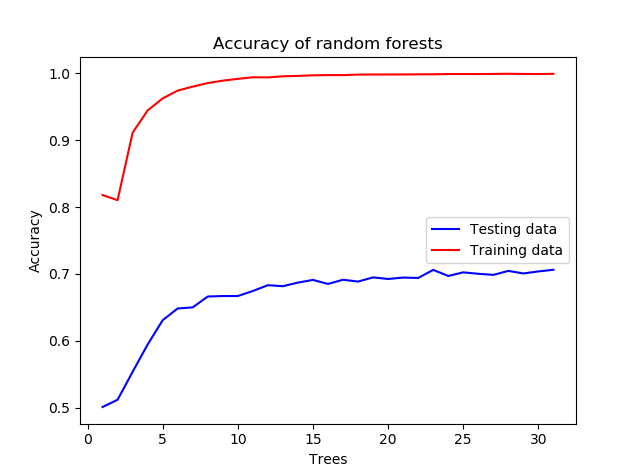
\includegraphics[scale=.7]{images/32treesAcc}\\
So more trees provides a better accuracy. But the classifier starts to have a decent accuracy after 10 trees.

\subsection{Difference in number of max\_features}
Here is a plot on how well the accuracy is using different numbers as max\_features:\\
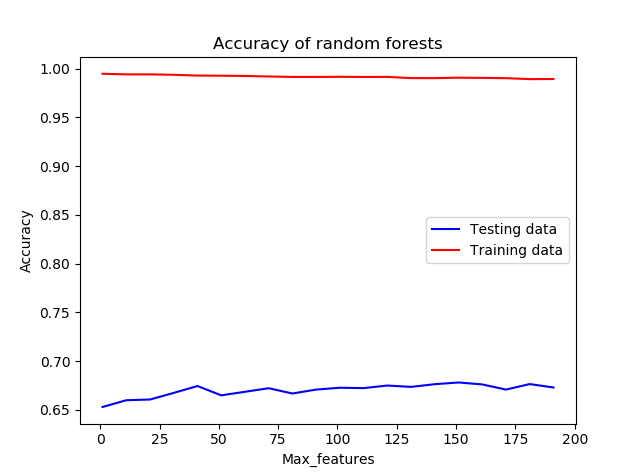
\includegraphics[scale=.7]{images/Max_featuresplot}\\
The number of trees used is 10.\\
\\
The default in the scikitlearn classifier is using the root of the number of all the features as max\_features. Since we have approximately 2000 features, the root becomes 44.72. That's why I computed different accuracies around this number.\\
\\
The plot tells us that it doesn't seem to matter much what we use as max\_features. The optimum in the plot is around 40 which gives us just more reason to stick with the default of using the root of all the features as max\_features.




\end{document}
